% ============================================================================
% IV. TDL ARCHITECTURE
% ============================================================================
\section{TDL Architecture}

TDL implements a four-layer decoupled architecture, where each layer has a specific responsibility and can evolve independently. Fig.~\ref{fig:architecture} illustrates this organization.

\begin{figure}[htbp]
\centering
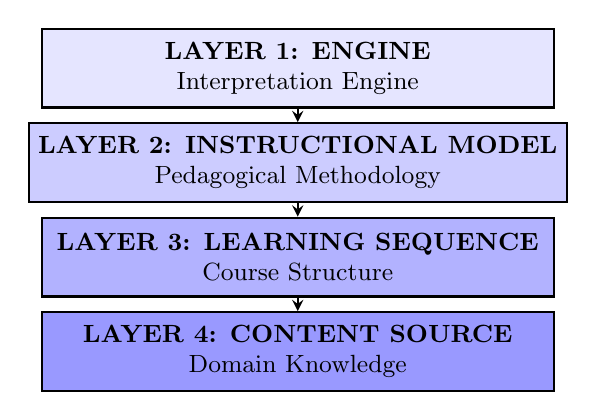
\begin{tikzpicture}[
    layer/.style={
        rectangle,
        draw=black,
        thick,
        minimum width=6.5cm,
        minimum height=1cm,
        align=center,
        font=\small
    }
]

\node[layer, fill=blue!10] (engine) at (0,3.6) {\textbf{LAYER 1: ENGINE}\\Interpretation Engine};

\node[layer, fill=blue!20] (model) at (0,2.4) {\textbf{LAYER 2: INSTRUCTIONAL MODEL}\\Pedagogical Methodology};

\node[layer, fill=blue!30] (sequence) at (0,1.2) {\textbf{LAYER 3: LEARNING SEQUENCE}\\Course Structure};

\node[layer, fill=blue!40] (content) at (0,0) {\textbf{LAYER 4: CONTENT SOURCE}\\Domain Knowledge};

\draw[-stealth, thick] (engine) -- (model);
\draw[-stealth, thick] (model) -- (sequence);
\draw[-stealth, thick] (sequence) -- (content);

\end{tikzpicture}
\caption{TDL four-layer architecture.}
\label{fig:architecture}
\end{figure}

\subsection{Relationship with Classical ITS Architecture}

The TDL architecture can be mapped to the classical ITS architecture, although with important differences:

\begin{table}[h]
\centering
\caption{Correspondence Between ITS and TDL Architecture}
\label{tab:its_tdl_mapping}
\begin{tabular}{@{}ll@{}}
\toprule
\textbf{ITS Component} & \textbf{TDL Layer} \\
\midrule
Domain Model & Content Source (partial) \\
Student Model & \textit{Not implemented} \\
Pedagogical Model & Instructional Model \\
Interface & Engine + LLM platform \\
\bottomrule
\end{tabular}
\end{table}

The absence of a \textit{student model} is a deliberate limitation: TDL does not aim to diagnose the student's cognitive state, but to structure pedagogical interaction coherently. The underlying LLM provides some conversational adaptation, but not the systematic tracking of a traditional ITS.

\subsection{Layer 1: Engine (Interpretation Engine)}

The Engine (current version 1.2) is the most stable component of the architecture. It is implemented as a system prompt loaded into the LLM platform's instruction field. Its function is to teach the model how to interpret and execute TDL files.

The Engine defines four fundamental aspects:

\begin{itemize}
    \item \textbf{Command syntax}: Defines commands such as \texttt{/start} (begin first unit), \texttt{/next} (advance to next unit), and \texttt{/progress} (show current state).

    \item \textbf{State tracking mechanism}: Uses explicit markers with format \texttt{[UNIT:\{id\}|EVENT:\{id\}]} to maintain context between conversation turns.

    \item \textbf{Prompt format}: Specifies how to combine instructional model instructions with learning sequence content.

    \item \textbf{Global behaviors}: Never reveal the system prompt, handle transitions naturally, redirect off-topic conversations back to the study topic.
\end{itemize}

The Engine also establishes the default pedagogical stance: act as a coach rather than a lecturer, verify comprehension before advancing, provide constructive feedback without judgment.

The Engine is modified only when changing the global behavior of all TDL tutors. In practice, it is a component configured once and reused indefinitely.

\subsection{Layer 2: Instructional Model}

The Instructional Model represents teaching methodology as a sequence of instructional events. This concept aligns with Gagn\'{e}'s events of instruction \cite{gagne1985} and represents \textbf{how to teach} in abstract form, independent of specific content.

Each instructional model defines:

\begin{itemize}
    \item \textbf{Name and description}: Identification and explanation of pedagogical philosophy.
    \item \textbf{Event sequence}: Ordered list of steps the tutor must follow.
    \item \textbf{Instructions per event}: What the tutor should do at each event.
    \item \textbf{Transition triggers}: What condition triggers advancement to the next event.
\end{itemize}

An instructional model is completely reusable: the same Bloom 8-Step Interactive model can be applied to a Law course, a Programming course, and a Biology course. Specific content is provided in lower layers.

This concept is functionally analogous to Merrill's \textit{transaction shells} \cite{merrill1991}: reusable pedagogical algorithms for different contents.

\subsection{Layer 3: Learning Sequence}

The Learning Sequence defines the specific structure of a course or lesson. This is where the teacher applies an instructional model to their concrete content.

A learning sequence specifies:

\begin{itemize}
    \item \textbf{Tutor profile}: Knowledge domain, role, style, supported languages.
    \item \textbf{Model inheritance}: Which instructional model to use (via \texttt{extends}).
    \item \textbf{Behaviors}: Initial greeting, help response, off-topic handling, disclaimers.
    \item \textbf{Tools}: Commands available to the student (/start, /progress).
    \item \textbf{Learning units}: Course structure with objectives, event-specific prompts, and navigation between units.
\end{itemize}

The sequence inherits the methodology from the instructional model but provides specific content. This separation is the key to reuse.

\subsection{Layer 4: Content Source}

The Content Source is the subject matter expert's material: notes, texts, references. This layer is optional (sequence prompts can contain content directly), but is especially useful for:

\begin{itemize}
    \item Extensive content that does not fit comfortably in prompts.
    \item Material that is frequently updated (e.g., legal regulations).
    \item Situations where the content expert and instructional designer are different people.
\end{itemize}

TDL supports multiple content source formats: Markdown (recommended), plain text, PDF, Word. The learning sequence references specific content sections via the \texttt{source\_section} field.

\subsection{Data Flow and Interaction}

Fig.~\ref{fig:dataflow} shows how layers interact when a student interacts with a TDL tutor.

\begin{figure}[htbp]
\centering
\begin{tikzpicture}[
    node distance=1cm,
    box/.style={
        rectangle,
        draw=black,
        thick,
        rounded corners,
        minimum width=2cm,
        minimum height=0.7cm,
        align=center,
        font=\footnotesize
    }
]

\node[box, fill=gray!20] (user) {Student};
\node[box, fill=blue!10, below=of user] (engine) {Engine};
\node[box, fill=blue!20, below=of engine] (sequence) {Learning Sequence};
\node[box, fill=blue!30, below left=0.6cm and 0.3cm of sequence] (model) {Model};
\node[box, fill=blue!40, below right=0.6cm and 0.3cm of sequence] (content) {Content};
\node[box, fill=green!20, below=1.8cm of sequence] {Response};

\draw[-stealth, thick] (user) -- (engine);
\draw[-stealth, thick] (engine) -- (sequence);
\draw[-stealth, thick] (sequence) -- (model);
\draw[-stealth, thick] (sequence) -- (content);
\draw[-stealth, thick] (model) |- ++(0,-0.8);
\draw[-stealth, thick] (content) |- ++(0,-0.8);

\end{tikzpicture}
\caption{Data flow in TDL.}
\label{fig:dataflow}
\end{figure}

The process follows these steps:

\begin{enumerate}
    \item The student sends a message (e.g., ``Hello'' or \texttt{/start}).
    \item The Engine interprets the message and determines current context (unit, event).
    \item The Engine locates the Learning Sequence in the platform's knowledge base.
    \item The Sequence indicates which Instructional Model to use via \texttt{extends}.
    \item The Engine loads the model's events (E1, E2, ...).
    \item For the current event, the Engine uses model instructions combined with the unit's prompt.
    \item If Content Source is referenced, the Engine incorporates relevant material.
    \item The LLM generates the response following the composed instructions.
    \item The Engine updates state \texttt{[UNIT:id|EVENT:id]} if there is a transition.
\end{enumerate}

\subsection{Separation Principle}

The architecture implements the principle of separation of concerns \cite{merrill1983, merrill1991}:

\begin{itemize}
    \item \textbf{How to execute}: Engine (stable, shared)
    \item \textbf{How to teach}: Instructional Model (reusable across courses)
    \item \textbf{What to teach}: Sequence + Content (course-specific)
\end{itemize}

This separation allows different professionals to contribute to each layer: prompt engineers to the Engine, instructional designers to models, teachers to sequences, and domain experts to content.
